\definecolor{grey95}{rgb}{0.98,0.98,0.98}

\newcommand{\ts}[1]{\text{\scriptsize{#1}}}
\newcommand{\tsi}[2]{\text{\scriptsize{#1}$_{#2}$}}
%\newcommand{\tsi}[2]{\text{\scriptsize{#1}}$_{\text{\tiny{#2}}}$}


\newcommand{\bal}[1]{\pscircle[fillstyle=solid,fillcolor=white](0.28,0.08){0.38}{#1}}
\newcommand{\bala}[1]{\pscircle[fillstyle=solid,fillcolor=white](0.12,0.10){0.3}{#1}}
\newcommand{\balb}[1]{\pscircle[fillstyle=solid,fillcolor=white](0.22,0.09){0.34}{#1}}
\newcommand{\balc}[1]{\pscircle[linewidth=0.5pt,linestyle=dashed,dash=2pt 1pt,
	fillstyle=solid,fillcolor=white](0.16,0.10){0.3}{#1}}
\newcommand{\bald}[1]{\pscircle[linewidth=0.5pt,linestyle=dashed,dash=2pt 1pt,
	fillstyle=solid,fillcolor=white](0.32,0.06){0.38}{#1}}
\newcommand{\bale}[1]{\pscircle[fillstyle=solid,fillcolor=white](0.07,0.08){0.25}{\scriptsize{#1}}}
\newcommand{\balf}[1]{\pscircle[fillstyle=solid,fillcolor=white](0.12,0.08){0.25}{\scriptsize{#1}}}

%\newcommand{\head}[1]{\psellipse[dimen=inner,fillstyle=none]
%	(0.5,0.1)(0.66,0.36){#1}}
\newcommand{\headpos}[1]{\pspolygon[linewidth=0.25pt,linestyle=dashed,dash=2pt 1pt,
	dimen=inner,fillstyle=solid,fillcolor=grey95](-0.1,-0.30)(-0.1,0.50)(1.2,0.35)(1.2,-0.15){#1}} % e.g. valve
	
\newcommand{\headneg}[1]{\pspolygon[linewidth=0.25pt,linestyle=dashed,dash=2pt 1pt,
	dimen=inner,fillstyle=solid,fillcolor=grey95](-0.1,0.28)(-0.1,-0.05)(1.2,-0.15)(1.2,0.40){#1}} % e.g. pump


\newpsstyle{arrstylepipe}{linewidth=1.5pt,showpoints=false,
        arrows=->,arrowsize=5.0pt 0,arrowlength=2.0,arrowinset=0}
\newpsobject{pipe}{psline}{style=arrstylepipe}

\newpsstyle{arrstylecontrol}{linewidth=1.0pt,showpoints=false,
        arrows=->,arrowsize=3.0pt 0,arrowlength=1.5,arrowinset=0}
\newpsobject{setpoint}{psline}{style=arrstylecontrol}

\newpsstyle{sensorstyle}{linewidth=1.0pt,showpoints=false}
\newpsobject{sensor}{psline}{style=sensorstyle}
\newpsstyle{sensorstyledashed}{linewidth=1.0pt,showpoints=false,linestyle=dashed,dash=2pt 1pt}
\newpsobject{sensordashed}{psline}{style=sensorstyledashed}


%%% VALVE
\newcommand{\valve}[0]{
		\pspolygon[linewidth=1pt,fillstyle=solid,fillcolor=white]
			(-0.18,-0.18)(0.18,0.18)(-0.18,0.18)(0.18,-0.18)
		\psline[linewidth=2pt](0,0)(0.30,0)
		\pswedge[dimen=inner,fillstyle=solid,fillcolor=white](0.30,0){0.18}{-90}{90}
}
%%% RESISTANCE
\newcommand{\resistance}[0]{\pspolygon[linewidth=1pt,fillstyle=solid,fillcolor=black]
	(-0.18,-0.18)(0.18,0.18)(-0.18,0.18)(0.18,-0.18)}
\newcommand{\resistancesmall}[0]{\pspolygon[linewidth=1pt,fillstyle=solid,fillcolor=black]
	(-0.12,-0.12)(0.12,0.12)(-0.12,0.12)(0.12,-0.12)}
%%% PUMP
\newcommand{\pump}[0]{
	\pspolygon[linewidth=1.0pt,fillstyle=solid,fillcolor=white](-0.35,-0.5)(0,0)(0.35,-0.5)
	\pscircle[linewidth=1.0pt,fillstyle=solid,fillcolor=white](0,0){0.35}
}
%%% PID CONTROLLER
\newcommand{\pid}[1]{\psframe[dimen=middle,linewidth=0.5pt,fillstyle=solid,fillcolor=white]
	(-0.25,-0.25)(0.25,0.25)
	%\psline[linewidth=0.5pt](0,0.25)(-0.25,0)(0,-0.25)(-0.25,-0.25)(0.25,0.25)
	\rput(0,0){\ts{#1}}
	\setpoint(0,1.75)(0,0.25)}
\newcommand{\pidtop}[2]{\psframe[dimen=middle,linewidth=0.5pt,fillstyle=solid,fillcolor=white]
	(-0.25,-0.25)(0.25,0.25)\rput(0,0){\ts{#1}}
	\setpoint(0,0.7)(0,0.25)\rput(0,0.9){\ts{#2}}}
\newcommand{\pidleft}[2]{\psframe[dimen=middle,linewidth=0.5pt,fillstyle=solid,fillcolor=white]
	(-0.25,-0.25)(0.25,0.25)\rput(0,0){\ts{#1}}
	\setpoint(-0.7,0)(-0.25,0)\rput(-1.0,0){{\ts{#2}}}}


%\includegraphics[width=1.0\textwidth]{figs/CSTR_model.eps}

\begin{pspicture}(0,-1)(17,8)
%\psframe[linecolor=red](0,0)(17,8)
%\psgrid[subgriddiv=1,griddots=10,gridlabels=5pt](0,-1)(17,18)

%\definecolor{colour0}{rgb}{0.9,0.9,0.9}

% Pump
\rput(9.5,2.2){
	\rput(0.20,0.25){\pipe(0,0)(6.5,0)}
	\rput{90}(2.1,0.25){\resistance}
	\rput[b](2.1,0.6){\tsi{R}{1}}
	\rput[l](0.2,0.5){\ts{PP}}
	\rput[l](0.8,0.5){\tsi{FLOW}{2}}

	\psdot[dotscale=1.5](3.0,0.25)
	\pipe(3.0,0.25)(3.0,-2.0)
	\rput{0}(3.0,-1.0){\resistance}
	\rput[b](3.4,-1.1){\tsi{R}{2}}
	\rput(3.0,-2.3){\tsi{FLOW}{3}}

	\rput{90}(5.2,0.25){\resistance}
	\rput[l](6.8,0.25){\tsi{FLOW}{4}}


	\sensor(5.8,-0.8)(5.8,1.2)(6.9,1.2)
	\rput(5.8,-0.8){\bale{F}}
	\rput(5.8,1.7){\tsi{MEAS}{5}}
	\rput(5.85,1.2){\balf{\tsi{c}{A}}}
	%\rput(5.8,1.2){\balb{$c_{A}$}}
	\rput(6.9,1.2){\balf{\tsi{c}{B}}}
	\rput(6.9,1.7){\tsi{MEAS}{6}}
	\rput(5.8,-1.3){\tsi{MEAS}{9}}
	\pump
	%\rput[b](0.0,-1.0){$h^{\text{PU}}_{0},K^{\text{PU}}_{1},K^{\text{PU}}_{2}$}
	%\rput[b](0,-1.0){\headneg{$\Delta h^{\text{pump}}$}}
	%\rput(0,-0.9){$\Delta h^{\text{pump}}$}
	\psline[linewidth=1.5pt](0,0)(-1,0)
}

% CSTR
\rput(7,2){
	%Jacket
		% Level sensor
	\psframe[linecolor=black, linewidth=0.04, fillstyle=solid, dimen=outer, framearc=0.3](-2.1,-0.7)(1.2,1.75)
	\pipe(-6.2,1)(-2.1,1)
		% Flow inside jacket
	\psline[linewidth=1.5pt,linestyle=dotted,dotsep=0.05,linearc=0.1]
		(-2.1,1)(-1.8,1)(-1.8,-0.4)(0.4,-0.4)(0.4,-0.7)
	\rput{90}(-0.7,-0.4){\resistancesmall}
	\rput[b](-0.9,-0.9){\psTextFrame[fillstyle=solid,fillcolor=white,linecolor=white](0,0)(0.4,0.3){\tsi{R}{9}}}
	\pipe(0.4,-0.7)(0.4,-2.5)
	\rput{0}(0.4,-1.5){\resistance}
	\rput[B](0.9,-1.6){\tsi{R}{10}}
	\rput(0.4,-2.7){\tsi{FLOW}{8}}

	\rput{90}(-5,1){\resistance}
	\rput[b](-5.0,0.5){\tsi{R}{5}}
	\rput{90}(-3.4,1){\valve}
	\rput[b](-3.4,0.5){\tsi{R}{6}}
	\rput[l](-3.1,1.4){\tsi{V}{2}}

	\rput[l](-6.2,1.5){\tsi{T}{3}}
	\rput[l](-6.2,1.2){\ts{PCW}}
	\rput[r](-6.3,1.0){\tsi{FLOW}{5}}
	\sensor(-5.5,1.0)(-5.5,-0.0)(-6.5,-0.0)

	\rput(-5.5,-0.0){\bale{T}}
	\rput[l](-5.2,-0.0){\tsi{MEAS}{10}}
	\rput(-6.5,-0.0){\bale{P}}
	\rput(-6.5,-0.5){\tsi{MEAS}{11}}

	\pipe(-2.1,-0.2)(-3.4,-0.2)(-3.4,-1.4)
	\rput{90}(-2.8,-0.2){\resistance}
	\rput[b](-2.8,-0.7){\tsi{R}{8}}
	\rput(-3.4,-1.6){\tsi{FLOW}{7}}

	\rput(0.7,-0.30){\tsi{T}{4}}
	
	\psellipse[dimen=inner, linecolor=black, linewidth=0.04](0,2.75)(1.5,.5)
	\psframe[dimen=inner, linecolor=black, linewidth=0.04, fillstyle=solid](-1.5,0)(1.5,2.75)
	\psframe[dimen=outer, linecolor=black, linewidth=0.00,
		fillstyle=crosshatch, hatchwidth=0.01, hatchsep=1pt, hatchcolor=lightgray](-1.5,0)(1.5,2.0)
	\psframe[fillstyle=solid,fillcolor=black](1.5,2.15)(1.62,1.85)
	\psline[linewidth=1.0pt](1.5,2.0)(6.5,2.0)(6.5,0.5)
	\rput{90}(6.5,0.4){\valve}
	\rput[b](6.5,-0.1){\tsi{R}{3}}
	\rput[b](7.75,-0.1){\tsi{R}{4}}
	\rput[b](6.9,0.7){\tsi{V}{1}}
	% Level controller
	\rput(2.5,2.0){\bale{L}}
	%\rput{180}(3.8,2.0){\pid}
	\rput{0}(3.8,2.0){\pidtop{LC}{SP$_1$}}
	\rput(4.7,2.2){\tsi{CNT}{1}}

	\rput{90}(-1.52,0.5){\resistancesmall}\pipe(-1.52,0.5)(-0.9,0.5)
	\rput[l](-0.85,0.5){\tsi{FLOW}{6}}
	\rput[l](1.05,0.2){\ts{PB}}
	\rput[b](-1.75,0.70){\psTextFrame[fillstyle=solid,fillcolor=white,linecolor=white](0,0)(0.4,0.3){\tsi{R}{7}}}
	\rput(0.1,1.5){\tsi{T}{2}}
	\rput(-0.3,1.0){\tsi{c}{A}}
	\rput(0.3,1.0){\tsi{c}{B}}
	\rput(1.0,1.0){\tsi{c}{C}}
	\psellipse[fillstyle=solid,fillcolor=black](-0.9,1.5)(0.1,0.07)
	\sensor(-3.4,5.0)(-0.9,5.0)(-0.9,1.5)
	\rput(-0.9,5.0){\bale{T}}
	\rput(-0.1,5.0){\tsi{MEAS}{7}}
	% Temperature controller
	\sensor(-3.4,2.75)(-3.4,1.5) % Temperature controller to flow controller
	\sensor(-4.4,1)(-4.4,3)(-3.4,3)
	\rput{0}(-3.8,3.6){\tsi{SP}{3}}
	\rput{0}(-3.4,5.0){\pidleft{TC}{\tsi{SP}{2}}}
	\rput{0}(-3.4,3.0){\pid{\ts{FC}}}
	\rput(-4.4,2.0){\bale{F}}
	\rput(-5.1,2.2){\tsi{MEAS}{8}}
	\sensordashed(-3.4,4.0)(-2.8,4.0)
	\rput(-3.8,4.4){\tsi{CNT}{2}}
	\rput(-2.6,4.0){\bale{S}}
	\rput(-2.55,4.4){\tsi{MEAS}{14}}
	\sensordashed(-3.4,2.0)(-2.8,2.0)
	\rput{90}(-3.55,2.0){\tsi{CNT}{3}}
	\rput(-2.55,2.4){\tsi{MEAS}{13}}
	\rput(-2.6,2.0){\bale{S}}
% Cascade controller outline
%	\pspolygon[linewidth=0.5pt,linestyle=dashed,dash=2pt 1pt,linearc=0.0]
%		(-5.0,2.6)(-5.0,5.6)(-1.8,5.6)(-1.8,2.6)
	
	\pipe(5,4.5)(0.9,4.5)(0.9,3.16)
	\rput[r](6.0,4.5){\tsi{FLOW}{1}}
	\rput[r](5.0,4.2){\tsi{T}{1}}
	\rput[r](5.0,3.9){\tsi{c}{A0}}
	
	\sensor(3.8,5.5)(1.8,5.5)(1.8,4.5)
	\rput(1.0,5.5){\tsi{MEAS}{2}}
	\rput(1.8,5.5){\bale{F}}
	\rput(2.8,5.9){\tsi{MEAS}{3}}
	\rput(2.8,5.5){\bale{T}}
	\rput(3.8,5.5){\bale{C}}
	\rput(4.6,5.5){\tsi{MEAS}{1}}
	
	\sensordashed(5.6,2.6)(5.6,2.0)
	\rput(5.6,2.6){\bale{S}}
	\rput(6.4,2.6){\tsi{MEAS}{12}}
	\rput(2.5,2.5){\tsi{MEAS}{4}}
}

%\rput(7,2){
%}

\end{pspicture}
